\begin{enumerate}
\item M and N are two points on the X axis and Y axis respectively.\\
      P \brak{3,2} divides the line segment MN in the ratio $2:3$.\\
      Find.
		\begin{enumerate}
		\item the coordinates of M and N
		\item slope of the line MN
		\end{enumerate}

\item The vertices of a $\triangle{ABC}$ are $A\brak{3,8}$,$B\brak{-1,2}$ and $C\brak{6,-6}$.Find:
\begin{enumerate}
    \item Slope of $BC$
    \item Equation of a line perpendicular to $BC$ and passing through $A$.
\end{enumerate}

\item Use ruler and compass only for answering this question. 
Draw a circle of radius $4$$\mathrm{cm}$. Mark the centre as O. Mark a point P outside the circle at a distance of $7$$\mathrm{cm}$ from the centre. Construct two tangents to the circle from the external point P. 
Measure and write down the length of any one tangent.

\item Using ruler and a compass only, construct a semi-circle with diameter $BC = $7$\mathrm{cm}$. 
Locate a point $A$ on the circumference of the semicircle such that $A$ is equidistant from $B$ and $C$. Complete the cyclic quadrilateral $ABCD$, such that $D$ is equidistant from $AB$ and $BC$. Measure $\angle ADC$ and write it down.

\item In the given figure $AC$ is a tangent to the circle with center $O$.
If $\angle{ADB}=55\degree$,find $x$ and $y$.Give reasons for your answers.

\begin{figure}[!ht]
		\centering
		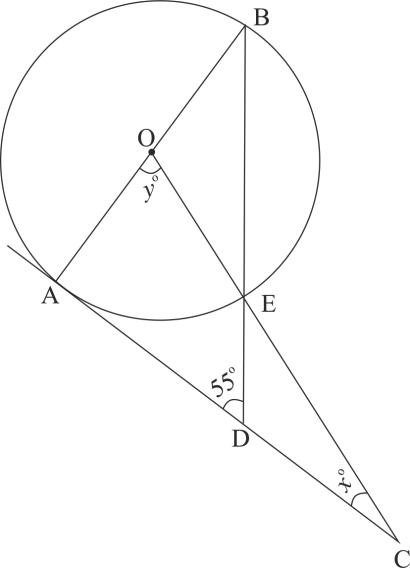
\includegraphics[width=\columnwidth]{figs/icse3.jpg}
		\caption{}
		\label{fig:enter-label}
	\end{figure}

\item In the given figure ,$ABCDE$ is a pentagon inscribed in a circle such that $AC$ is a diameter and side $BC$ $\slash \slash$ $ AE $.If $\angle  BAC $=$50\degree$,find giving reasons:
\begin{enumerate}
    \item $\angle ACB$
    \item $\angle EDC$
    \item $\angle BEC$
\end{enumerate}
\text Hence prove that $BE$ is also a diameter
\begin{figure}[!ht]
		\centering
		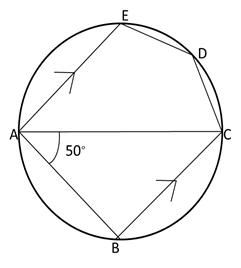
\includegraphics[width=\columnwidth]{figs/icse4.jpg}
		\caption{}
		\label{fig:enter-label}
\end{figure}

\item In the given figure ,$\angle{PQR}$=$\angle{PST}$=$ 90\degree$,$PQ=$5$\mathrm{cm}$.and $PS=$2$\mathrm{cm}$.
\begin{enumerate}
    \item Prove that $\triangle{PQR}$  $\sim$   $\triangle{PST}$.
    \item Find Area of $\triangle{PQR}$: Area of quadrilateral $SRQT$.
\end{enumerate}

\begin{figure}[!ht]
		\centering
		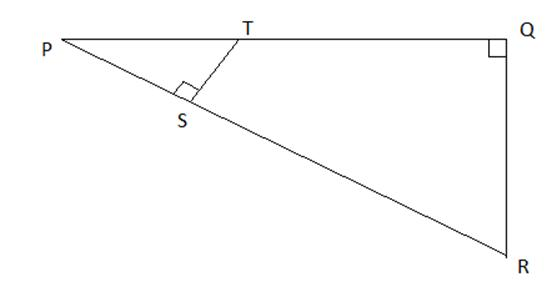
\includegraphics[width=\columnwidth]{figs/icse1.jpg}
		\caption{}
		\label{fig:enter-label}
\end{figure}
\end{enumerate}
	
